\documentclass{beamer}
\usepackage[english,russian]{babel}
\usepackage[utf8]{inputenc}
\usepackage{amsmath}
\usepackage{hyperref}
\usetheme{Warsaw}
\usepackage{listings}
\usepackage{xcolor}
\usepackage{tikz}
\usetikzlibrary{graphs}
\usepackage{algpseudocode}

\lstset{
    frame=tb,
    tabsize=4,
    showstringspaces=false,
    numbers=left,
    commentstyle=\color{green},
    keywordstyle=\color{blue},
    stringstyle=\color{red},
    emph={baz},
    emphstyle=\textbf
}

\begin{document}

\title{SAT/SMT solvers\newline  7. Pointer Logic}
\author{Roman Kholin}
\institute{Lomonosov Moscow State University}
\date{Moscow, 2023}

\begin{frame}
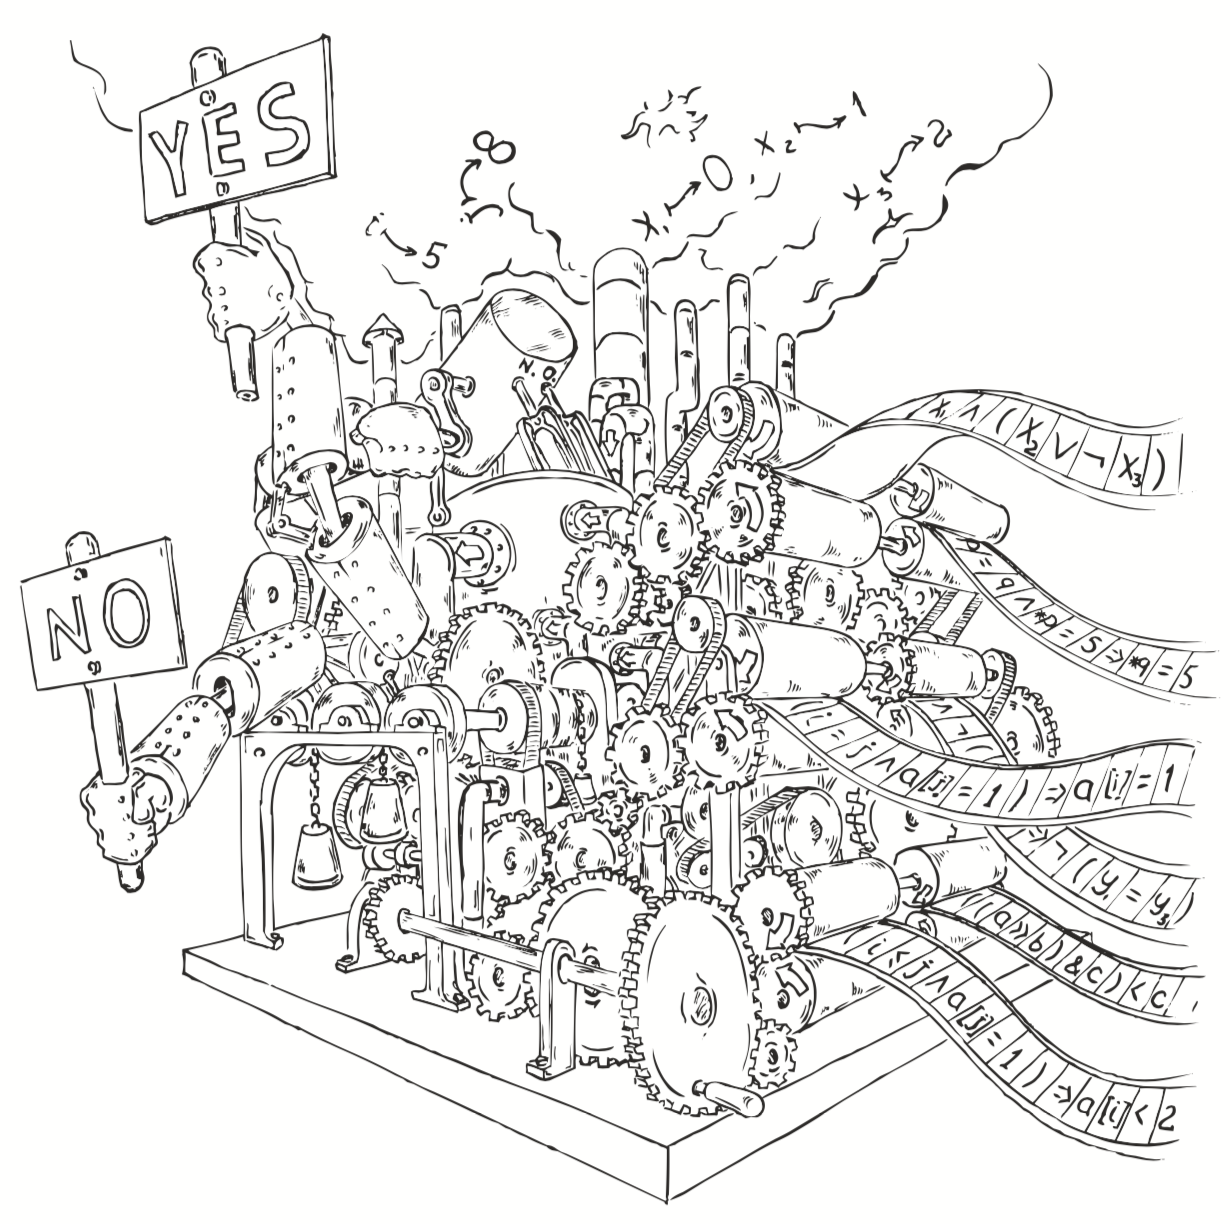
\includegraphics[scale=0.5]{../decision-procedure.png}
\end{frame}

\frame{\titlepage}

\begin{frame}{Definitions}
\begin{block}{Memory model}
A memory model describes the assumptions that are made about the way memory cells are addressed. We assume that the architecture provides a continuous, uniform address space, i.e., the set of addresses A is a subinterval of the integers $\{0, \dots, N - 1\}$. Each address corresponds to a memory cell that is able to store one data word. The set of data words is denoted by $D$. A $memory$ $valuation$ $M : A \rightarrow D$ is a mapping from a set of addresses $A$ into the domain $D$ of data words
\end{block}
\begin{block}{Memory layout}
A memory layout $L : V \rightarrow A$ is a mapping from each variable $v \in V$ to an address $a \in A$. The address of $v$ is also called the memory location of $v$
\end{block}
\end{frame}

\begin{frame}{Example}
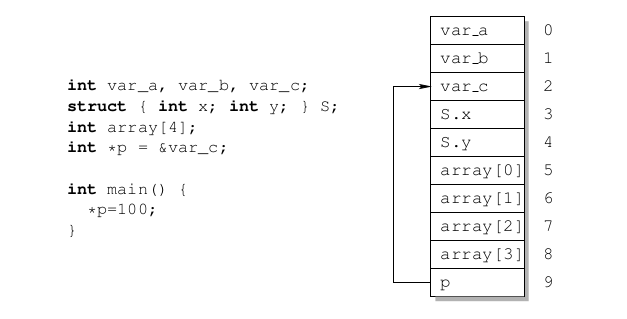
\includegraphics[scale=0.5]{layout.png}
\end{frame}

\begin{frame}{Analysis of programs with pointers}
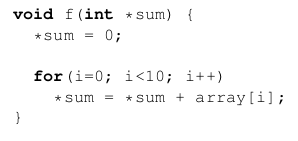
\includegraphics[scale=0.5]{ex1.png}
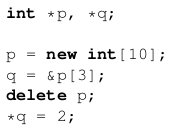
\includegraphics[scale=0.5]{ex2.png}
\end{frame}

\begin{frame}{Definitions}
\begin{block}{Pointer logic}
\begin{itemize}
\item $formula: formula \wedge formula$ | $\lnot formula$ | $(formula)$ | $atom$
\item $pointer = pointer$ | $term = term$ | $pointer < pointer$ | $term < term$
\item $pointer : pointer$-$identifier$ | $pointer + term$ | $(pointer)$ | $\&identifier$ | $\&*pointer$ | $pointer$ | NULL
\item $term : identifier$ | $*pointer$ | $term$ $op$ $term$ | $(term)$ | $integer$-$constant$ | $identifier[term]$
\item $op : +$ | $-$
\end{itemize}
\end{block}
\end{frame}

\begin{frame}{Example}
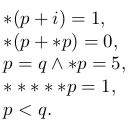
\includegraphics[scale=0.5]{perm.png}
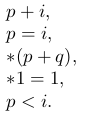
\includegraphics[scale=0.5]{not_perm.png}
\end{frame}

\begin{frame}{Semantics}
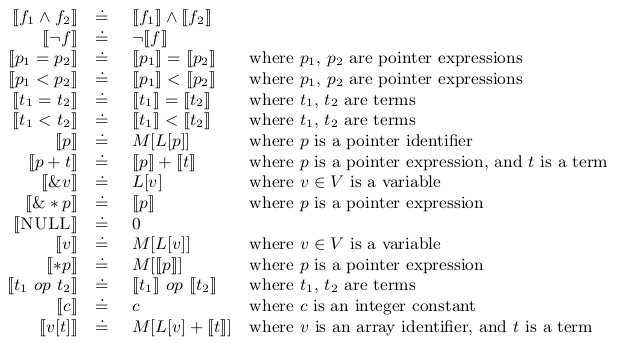
\includegraphics[scale=0.5]{semantics.png}
\end{frame}

\begin{frame}{Example}
$*((\&a) + 1) = a[1]$
\end{frame}

\begin{frame}{Example}
$*((\&a) + 1) = a[1]$
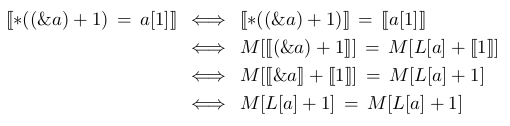
\includegraphics[scale=0.5]{semantics_ex.png}
\end{frame}

\begin{frame}{Definitions}
\begin{block}{Memory Model Axiom 1 (<<No object has address 0>>)}
The fact <<no object has address 0>> is easily formalized:\newline
$\forall v \in V.L[v] \ne 0$
\end{block}
\begin{block}{Memory Model Axiom 2 (<<Objects have size at least one>>)}
The fact <<an object has size at least one>> is easily captured by\newline
$\forall v \in V.\sigma(v) \ge 1$
\end{block}
\begin{block}{Memory Model Axiom 3 (<<Objects do not overlap>>)}
Different objects do not share any addresses:\newline
$\forall v_1, v_2 \in V.v_1 \ne v_2 \Rightarrow \{L[v_1], \dots, L[v_1] + \sigma(v1) - 1\} \cap \{L[v_2], \dots, L[v_2] + \sigma(v_2) - 1\} = \emptyset$
\end{block}
\end{frame}

\begin{frame}{Adding structure types}
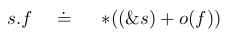
\includegraphics[scale=0.5]{struct1.png}\newline
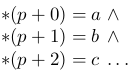
\includegraphics[scale=0.5]{struct2.png}\newline
\end{frame}

\begin{frame}{A decision procedure}
\begin{itemize}
\item The logic of pointers is reduced to the logic of arrays
\item The formulas generated by this semantic translation contain array read operators and linear arithmetic over the type that is used for the indices
\item Problem - quantors
\end{itemize}
\end{frame}

\begin{frame}{Example}
$p = \&x \wedge x = 1 \Rightarrow *p = 1$\newline
\end{frame}

\begin{frame}{Example}
$p = \&x \wedge x = 1 \Rightarrow *p = 1$\newline
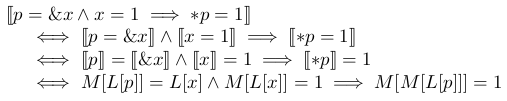
\includegraphics[scale=0.5]{ex_good.png}\newline
\end{frame}

\begin{frame}{Example}
$p \rightarrow x \Rightarrow p = \&x$\newline
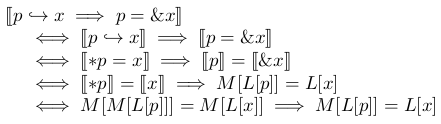
\includegraphics[scale=0.5]{ex_bad1.png}\newline
\end{frame}

\begin{frame}{Example}
$p \rightarrow x \Rightarrow p = \&x$\newline
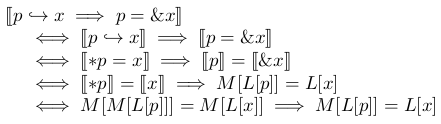
\includegraphics[scale=0.5]{ex_bad1.png}\newline
\end{frame}

\begin{frame}{Example}
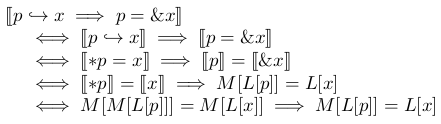
\includegraphics[scale=0.5]{ex_bad1.png}\newline
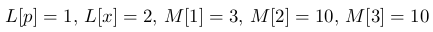
\includegraphics[scale=0.5]{ex_bad2.png}\newline
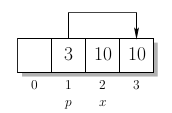
\includegraphics[scale=0.5]{ex_bad3.png}\newline
\end{frame}

\begin{frame}{Applying the Memory model axioms}
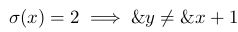
\includegraphics[scale=0.5]{meory1.png}\newline
\end{frame}

\begin{frame}{Applying the Memory model axioms}
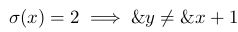
\includegraphics[scale=0.5]{meory1.png}\newline
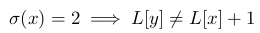
\includegraphics[scale=0.5]{meory2.png}\newline
\end{frame}

\begin{frame}{Applying the Memory model axioms}
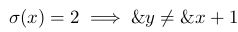
\includegraphics[scale=0.5]{meory1.png}\newline
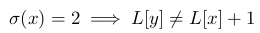
\includegraphics[scale=0.5]{meory2.png}\newline
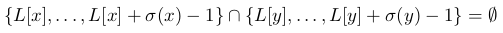
\includegraphics[scale=0.5]{meory3.png}\newline
\end{frame}

\begin{frame}{Applying the Memory model axioms}
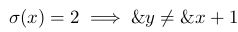
\includegraphics[scale=0.5]{meory1.png}\newline
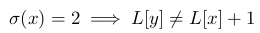
\includegraphics[scale=0.5]{meory2.png}\newline
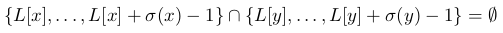
\includegraphics[scale=0.5]{meory3.png}\newline
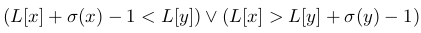
\includegraphics[scale=0.5]{meory4.png}\newline
\end{frame}

\begin{frame}{Applying the Memory model axioms}
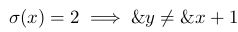
\includegraphics[scale=0.5]{meory1.png}\newline
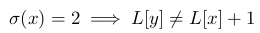
\includegraphics[scale=0.5]{meory2.png}\newline
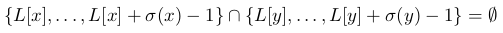
\includegraphics[scale=0.5]{meory3.png}\newline
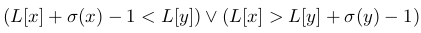
\includegraphics[scale=0.5]{meory4.png}\newline
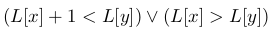
\includegraphics[scale=0.5]{meory5.png}\newline
\end{frame}

\begin{frame}{Pure variables}
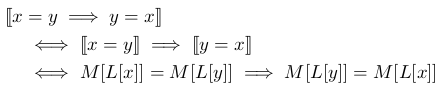
\includegraphics[scale=0.5]{ex_pure.png}\newline
\end{frame}

\begin{frame}{Pure variables}
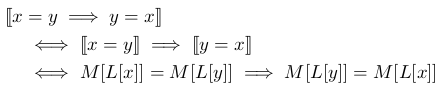
\includegraphics[scale=0.5]{ex_pure.png}\newline
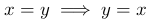
\includegraphics[scale=0.5]{ex_pure2.png}\newline
\end{frame}

\begin{frame}{Pure variables}
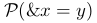
\includegraphics[scale=0.5]{pure1.png}\newline
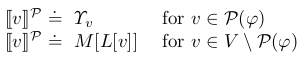
\includegraphics[scale=0.5]{pure2.png}\newline
\end{frame}

\begin{frame}{Pure variables}
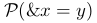
\includegraphics[scale=0.5]{pure1.png}\newline
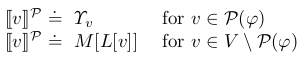
\includegraphics[scale=0.5]{pure2.png}\newline
Theorem:\newline
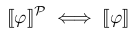
\includegraphics[scale=0.5]{theorem.png}\newline
\end{frame}

\begin{frame}{Partitioning the Memory}
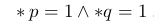
\includegraphics[scale=0.5]{partitioning1.png}\newline
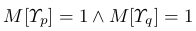
\includegraphics[scale=0.5]{partitioning2.png}\newline
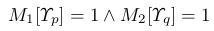
\includegraphics[scale=0.5]{partitioning3.png}\newline
\end{frame}

\begin{frame}{Partitioning the Memory}
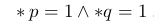
\includegraphics[scale=0.5]{partitioning1.png}\newline
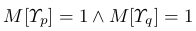
\includegraphics[scale=0.5]{partitioning2.png}\newline
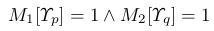
\includegraphics[scale=0.5]{partitioning3.png}\newline
Not always can be used:\newline
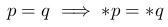
\includegraphics[scale=0.5]{partitioning4.png}\newline
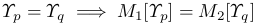
\includegraphics[scale=0.5]{partitioning5.png}\newline
\end{frame}

\begin{frame}
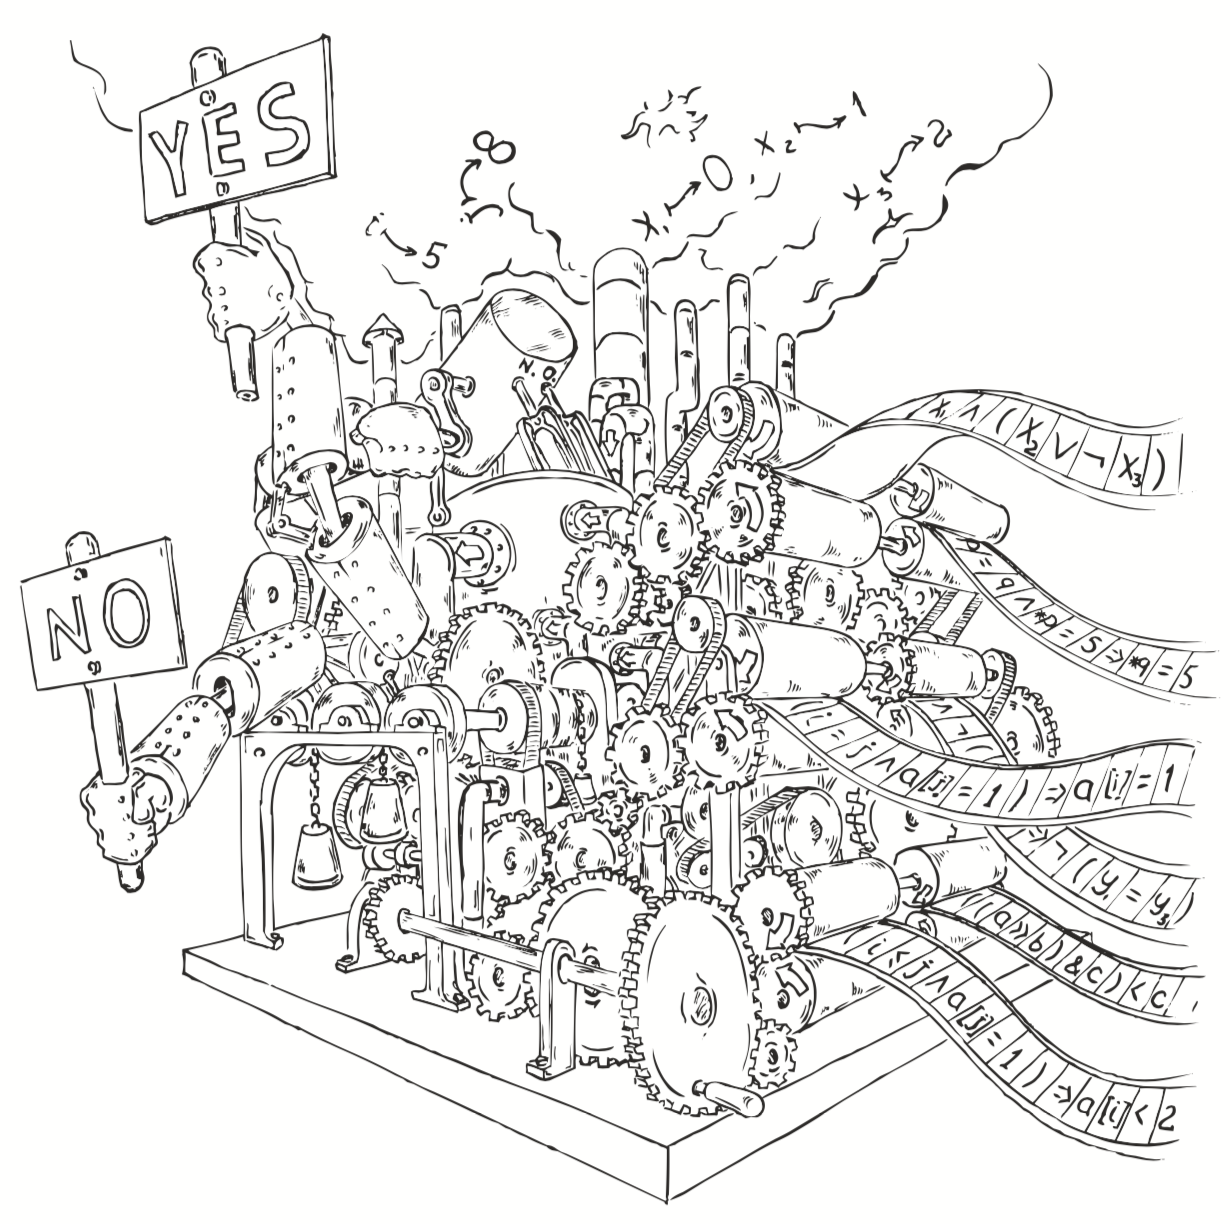
\includegraphics[scale=0.5]{../decision-procedure.png}
\end{frame}

\end{document}
